\section{Rota de estudo na danca de salão}
\label{sec:dance-elements-processo}
Nesta seção é presentada uma proposta de rota de estudo para o aprendizado da
dança de salão. 
Como mostra a Figura \ref{fig:dance-elements-processo},
a proposta está basejada em 3 níveis de trabalho.
\begin{figure}[!h]
\centering
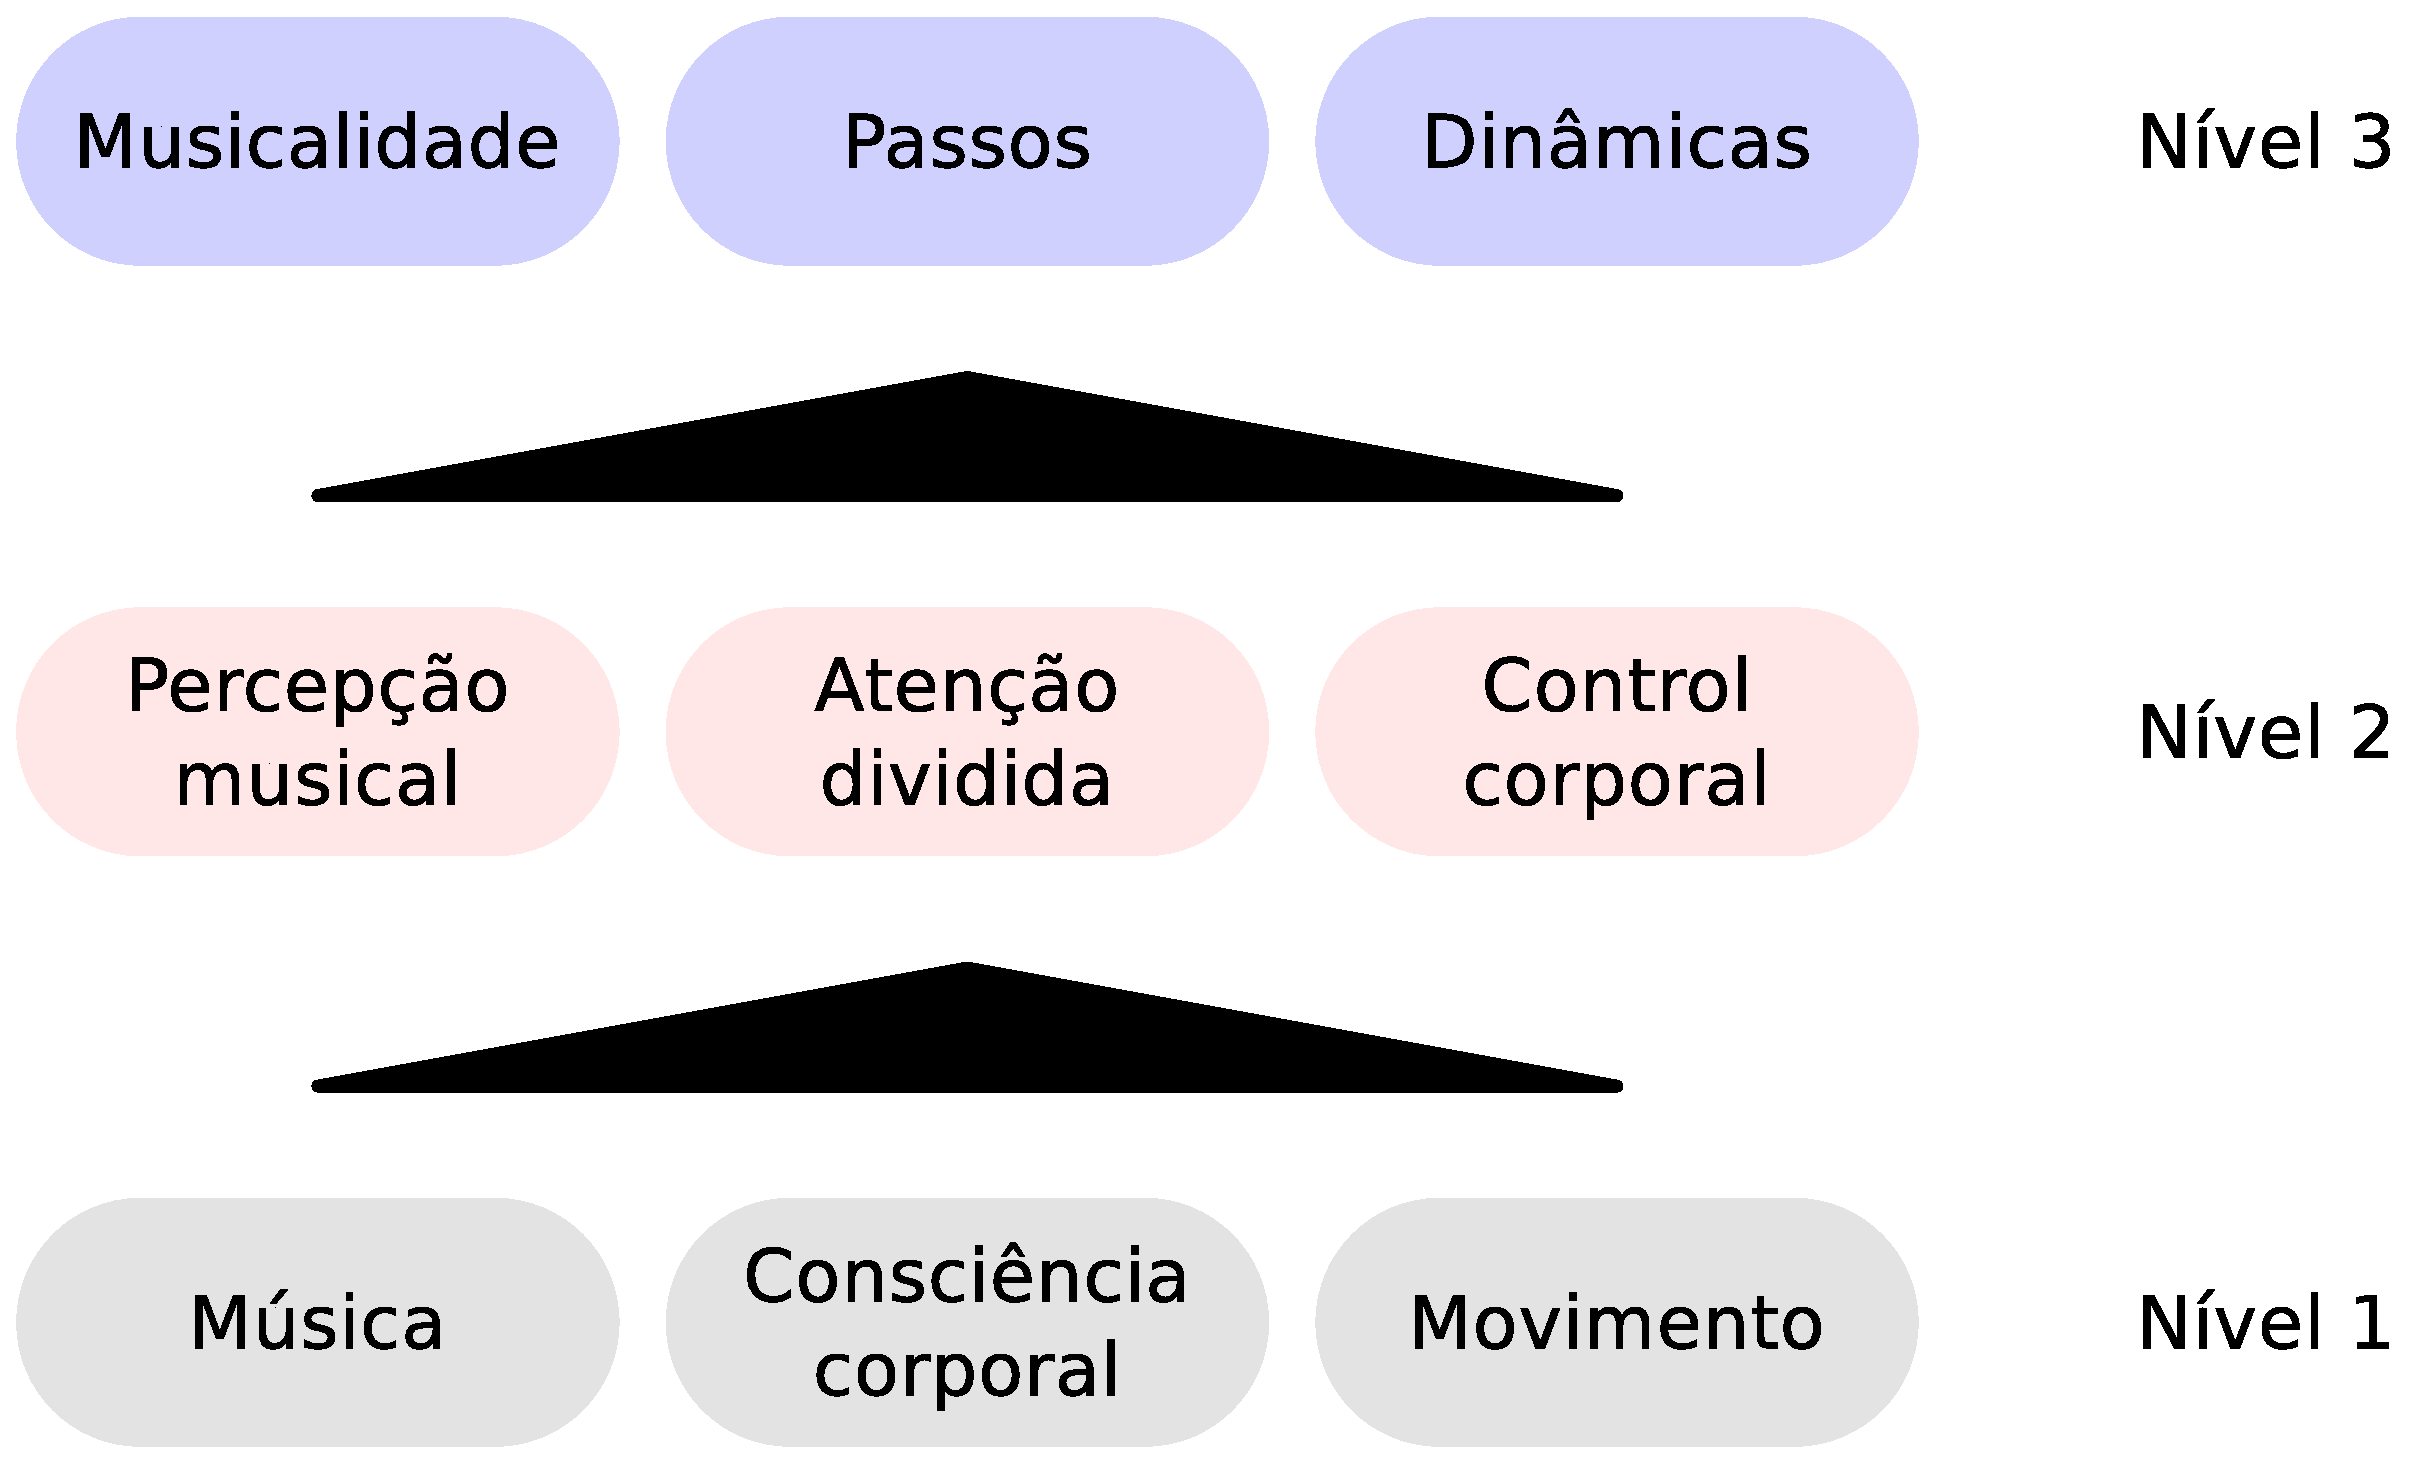
\includegraphics[width=0.7\textwidth]{chapters/cap-dance-elements/Diagrama-danca.eps}
\caption{Rota de estudo para o aprendizado da dança de salão.}
\label{fig:dance-elements-processo}
\end{figure}
\begin{itemize}
\item No nível 1 temos os temas mais básicos a serem estudados quando
iniciamos nosso percorrido na dança, estes são:
A teoria musical, a qual pode ser vista nos 
Capitulos \ref{cap:musicabasica}, \ref{cap:musicacomposer} e \ref{cap:musicatopicos}.
A consciência corporal, que é estudada no Capítulo \ref{fig:bodyrelations}.
O movimento, que corresponde ao aprimoramento de nossa aptidão física.
\item No nível 2 se inicia o perfeicionamento de habilidades,
mediante a combinação de vários componentes aprendidos no nível 1, estes são:
A percepção musical, a qual é vista no Capítulo \ref{cap:percepcaomusical}.
O controle corporal, que é estudado no Capítulo \ref{fig:bodyrelations}.
A atenção dividida, que é estudada nos Capítulos \ref{cap:aprendizagem} e \ref{chap:trainingbodycontrol}.
\item No nível 3 são listados os temas mais complexos os quais
requerem conhecimentos do nível 1 e/ou 2 para serem satisfatoriamente completados,
estes são:
A musicalidade, a qual é vista nos Capítulos \ref{chap:FundamentosMusicalidade} e \ref{chap:TopicosMusicalidade}.
As dinâmicas nos movimentos, que são estudadas na Seção \ref{sec:musicalidade:dinamicas}.
Os passos de dança, que são listados no Capítulo \ref{chap:passos-samba-gafieira}.
\end{itemize}
A proposta de estudo da Figura \ref{fig:dance-elements-processo} não aponta a que 
todo mundo deva inciar no nível 1, 
pois, dependendo da experiencia de vida de cada pessoa, elas podem ter conhecimentos de itens
dispersos em vários níveis no momento de iniciar seu aprendizado na dança de salão.
Esta proposta só busca dar uma orientação ao fluxo de estudos de um entusiasta da dança de salão.
